% This file was created by tikzplotlib v0.9.8.
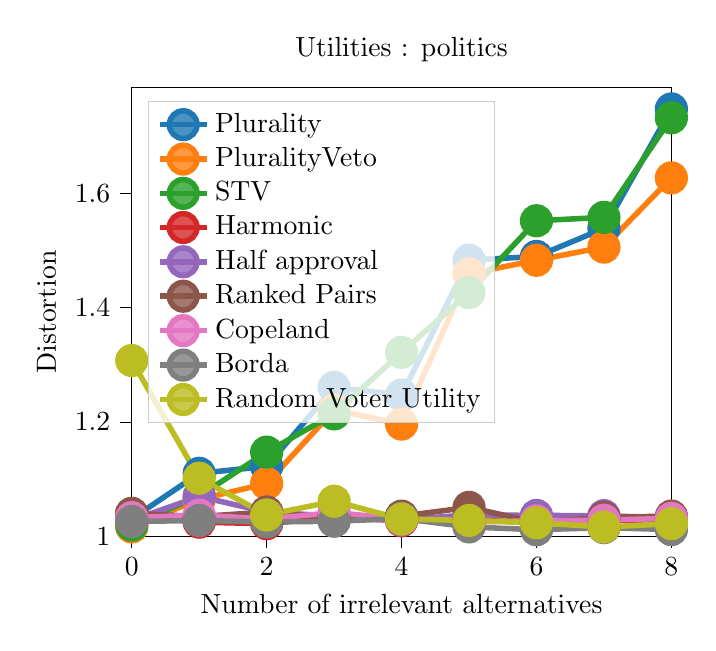
\begin{tikzpicture}

\definecolor{color0}{rgb}{0.12156862745098,0.466666666666667,0.705882352941177}
\definecolor{color1}{rgb}{1,0.498039215686275,0.0549019607843137}
\definecolor{color2}{rgb}{0.172549019607843,0.627450980392157,0.172549019607843}
\definecolor{color3}{rgb}{0.83921568627451,0.152941176470588,0.156862745098039}
\definecolor{color4}{rgb}{0.580392156862745,0.403921568627451,0.741176470588235}
\definecolor{color5}{rgb}{0.549019607843137,0.337254901960784,0.294117647058824}
\definecolor{color6}{rgb}{0.890196078431372,0.466666666666667,0.76078431372549}
\definecolor{color7}{rgb}{0.737254901960784,0.741176470588235,0.133333333333333}

\begin{axis}[
legend cell align={left},
legend style={
  fill opacity=0.8,
  draw opacity=1,
  text opacity=1,
  at={(0.03,0.97)},
  anchor=north west,
  draw=white!80!black
},
tick align=outside,
tick pos=left,
title={Utilities : politics},
x grid style={white!69.0196078431373!black},
xlabel={Number of irrelevant alternatives},
xmin=0, xmax=8,
xtick style={color=black},
y grid style={white!69.0196078431373!black},
ylabel={Distortion},
ymin=1, ymax=1.78401382462236,
ytick style={color=black}
]
\addplot [line width=2pt, color0, mark=*, mark size=5, mark options={solid}]
table {%
0 1.03034688615398
1 1.1099729674429
2 1.1221958223406
3 1.26036386041559
4 1.24690690331816
5 1.48282325765297
6 1.4891708560383
7 1.53816666078759
8 1.74721687290269
};
\addlegendentry{Plurality}
\addplot [line width=2pt, color1, mark=*, mark size=5, mark options={solid}]
table {%
0 1.01625628006108
1 1.06438302055516
2 1.09218439934773
3 1.22076898738076
4 1.19608147587155
5 1.45893918876447
6 1.48257788089865
7 1.50560353436685
8 1.62662742301375
};
\addlegendentry{PluralityVeto}
\addplot [line width=2pt, color2, mark=*, mark size=5, mark options={solid}]
table {%
0 1.01939582930462
1 1.07011817253686
2 1.1470425242806
3 1.21393807150532
4 1.32150579917911
5 1.42603880889523
6 1.5516482965486
7 1.55759851939875
8 1.73166649838503
};
\addlegendentry{STV}
\addplot [line width=2pt, color3, mark=*, mark size=5, mark options={solid}]
table {%
0 1.0397487244631
1 1.02456675269122
2 1.0218596953265
3 1.03299941735735
4 1.02696068887332
5 1.02986413625549
6 1.02262215523294
7 1.02889563137117
8 1.0266476330997
};
\addlegendentry{Harmonic}
\addplot [line width=2pt, color4, mark=*, mark size=5, mark options={solid}]
table {%
0 1.02774234194821
1 1.06948250221148
2 1.04230081685513
3 1.03508490798316
4 1.02849402680254
5 1.03747069053422
6 1.03631377846683
7 1.0359397334608
8 1.0317165660997
};
\addlegendentry{Half approval}
\addplot [line width=2pt, color5, mark=*, mark size=5, mark options={solid}]
table {%
0 1.03992149445234
1 1.03439413121123
2 1.04215646346133
3 1.03261654314017
4 1.03507601329209
5 1.05045738251676
6 1.02404126040326
7 1.03299251308378
8 1.03521972072978
};
\addlegendentry{Ranked Pairs}
\addplot [line width=2pt, color6, mark=*, mark size=5, mark options={solid}]
table {%
0 1.03248869748257
1 1.03691524010776
2 1.03012736003246
3 1.04139291899485
4 1.03020018768317
5 1.02499687927491
6 1.02677421669607
7 1.02803726198492
8 1.03129282369206
};
\addlegendentry{Copeland}
\addplot [line width=2pt, white!49.8039215686275!black, mark=*, mark size=5, mark options={solid}]
table {%
0 1.02569670960273
1 1.02748986067474
2 1.02493450552023
3 1.02612598381647
4 1.03087225705632
5 1.01625728151434
6 1.01127783850929
7 1.01497134447007
8 1.01156276954713
};
\addlegendentry{Borda}
\addplot [line width=2pt, color7, mark=*, mark size=5, mark options={solid}]
table {%
0 1.30717654585428
1 1.10138775718367
2 1.0371678231291
3 1.06114177299431
4 1.02992411546761
5 1.0276264988268
6 1.02351784064714
7 1.01616681423456
8 1.02193781062624
};
\addlegendentry{Random Voter Utility}
\end{axis}

\end{tikzpicture}
